This chapter provides relevant background for the $\mathcal{\mathcal{C} \mskip
-4mu \mathcal{E}}$ machine, outlining lambda calculus, evaluation strategies,
and Curien's calculus of closures.

\section{Preliminaries} \label{sec:prelim}

We begin with the simple lambda calculus ~\cite{barendregt1984lambda}:  $$ t::= x
\; | \;  \lambda x.t \; | \;  t \; t $$ where $x$ is a variable, $\lambda x.t$
is an abstraction, and $t \; t$ is an application. We also use lambda calculus
with deBruijn indices, which replaces variables with a natural number indexing
into the binding lambdas.  This calculus is given by the syntax: $$ t::= i \; |
\; \lambda t \; | \; t \; t $$ where $i \in \mathbb{N}$. In both cases, we use
the standard Barendregt syntax conventions, namely that applications are left
associative and the bodies of abstractions extend as far as possible to the
right ~\cite{barendregt1984lambda}.  A \emph{value} in lambda calculus refers to
an abstraction. We are concerned only with evaluation to weak head normal form
(WHNF), which terminates on an abstraction without entering its body.

In mechanical evaluation of expressions, it would be too inefficient to perform
explicit substitution. To solve this, the standard approach uses closures
~\cite{landin1964mechanical,curien1991abstract,jonesstg,biernacka2007concrete}.
Closures combine a term with an environment, which binds the free variables of
the term to closures. 

As the formal basis for closures we use Curien's calculus of
closures~\cite{curien1991abstract}, Figure~\ref{fig:calcclos}.  It is a
formalization of closures with an environment represented as a list of closures,
indexed by deBruijn indices. We will occasionally modify this calculus by
replacing the deBruijn indices with variables for readability, in which case
variables are looked up in the environment instead of indexed, e.g., $t[x = c, y
= c'])$ ~\cite{barendregt1984lambda}. We also add superscript and subscript
markers to denote unique syntax elements, e.g., $t', t_1 \in \textnormal{Term}$. 

\begin{figure}
\textbf{Syntax}
\begin{align*}
\tag{Term} t &::= i \; | \; \lambda t \; | \; t \; t  \\
\tag{Variable} i &\in \mathbb{N}  \\
\tag{Closure} c &::= t [\rho] \\
\tag{Environment} \rho &::= \bullet \; | \; c \cdot \rho \\
\end{align*}
\textbf{Semantics}
\begin{align*}
\tag{LEval}\inference
{t_1[\rho] {\xrightarrow{* }}_L \lambda t_2[\rho'] }
{t_1 t_3[\rho] \rightarrow_L t_2[t_3[\rho] \cdot \rho'] } 
\end{align*}
\begin{align*}
\tag{LVar} i [c_0 \cdot c_1 \cdot ... c_i \cdot \rho] \rightarrow_L c_i
\end{align*}
\caption{Curien's call-by-name calculus of closures ~\cite{curien1991abstract}}
\label{fig:calcclos}
\end{figure}

\section{Evaluation Strategies} \label{sec:eval}

There are three standard evaluation strategies for lambda calculus:
call-by-value, call-by-need, and call-by-name.  Call-by-value evaluates every argument
to a value, whereas call-by-need and call-by-name only evaluate an argument if
it is needed.  If an argument is needed more than once, call-by-name re-computes
the value, whereas call-by-need memoizes the value, so it is computed at most once.
Thus, call-by-need attempts to embody the best of both worlds---never repeat
work (call-by-value), and never perform unnecessary work (call-by-name). These
are intuitively good properties to have, and we illustrate the
correctness of such an intuition with the following example, modified from
~\cite{danvy2013synthetic}:


$$ \overbrace{c_m (c_m (\cdots(c_m}^{m} \; \mathit{id} \;
\overbrace{\mathit{id})\cdots) \mathit{id})}^{m} \; \mathit{true} \;
\mathit{id} \; \mathit{bottom} $$ where $c_n = \lambda s.\lambda z.\overbrace{s
\; (s \cdots (s}^{n} \; z) \cdots) $, $\mathit{true} = \lambda t.\lambda f.t$,
$\mathit{id}=\lambda x.x$, and \\ $\mathit{bottom} = (\lambda x.x \; x) \lambda x.x \; x$.
Call-by-value never terminates,
call-by-name takes exponential time, and call-by-need takes only polynomial time
~\cite{danvy2013synthetic}. Of course, this is a contrived example, but it
illustrates desirable properties of call-by-need.

In practice, however, there are significant issues with call-by-need evaluation.
We focus on the following: \emph{Delaying a computation is slower than
performing it immediately.} This issue is well known
\cite{johnsson1984efficient,jonesstg}, and has become part of the motivation
for \emph{strictness analysis}
\cite{mycroft1982abstract,wadler1987projections}, which transforms non-strict
evaluation to strict when possible.

\section{Existing Call-by-Need Machines}

Diehl et al. ~\cite{diehl2000abstract} review the call-by-need
literature in detail.  Here we summarize the most relevant points.

The best known machine for lazy evaluation is the Spineless Tagless
G-Machine (STG machine), which underlies the Glasgow Haskell Compiler (GHC). 
STG uses flat environments that can be allocated on the stack, the heap,
or some combination ~\cite{jonesstg}.  

Two other influential lazy evaluation machines relevant to the $\mathcal{\mathcal{C} \mskip -4mu \mathcal{E}}$
machine are the call-by-need Krivine machines
~\cite{lkm,krivine2007call,sestoft}, and the three-instruction machine (TIM)
~\cite{TIM}.  Krivine machines started as an approach to call-by-name
evaluation, and were later extended to call-by-need
~\cite{krivine2007call,sestoft,danvy2013synthetic,lkm}.  The $\mathcal{\mathcal{C} \mskip -4mu \mathcal{E}}$
modifies the lazy Krivine machine to capture the environment sharing given by
the cactus environment. The TIM is an implementation of call-by-need and
call-by-name ~\cite{TIM}.  It involves, as the name suggests, three machine
instructions, \texttt{TAKE}, \texttt{PUSH}, and \texttt{ENTER}. In
Section~\ref{sec:impl}, we follow Sestoft ~\cite{sestoft} and
re-appropriate these instructions for the $\mathcal{\mathcal{C} \mskip -4mu \mathcal{E}}$ machine.

There has also been recent interest in \emph{heapless} abstract
machines for lazy evaluation. Danvy et al. ~\cite{danvy2012inter} and
Garcia et al. ~\cite{garcia2009lazy} independently derived similar
machines from the call-by-need lambda calculus
~\cite{ariola1995call}. These are interesting approaches, but it is not yet
clear how these machines could be implemented efficiently.

\section{Formal Logic} \label{sec:background}

With recent improvements in higher order logics, machine verification of
algorithms has become a valuable tool in software development. Instead of
relying heavily on tests to check the correctness of programs, verification can
prove that algorithms implement their specification for \emph{all} inputs.
Implementing both the specification and the proof in a machine-checked logic
removes the vast majority of bugs found in hand-written proofs, ensuring far
higher confidence in correctness than other standard methods. Other approaches,
such as fuzz testing, have confirmed that verified programs remove effectively
all bugs \cite{yangfuzz}.

This approach applies particularly well to compilers. Often, the specification
for a compiler is complete: source level semantics for some languages are
exceedingly straightforward to specify, and target architectures have lengthy
specifications that are amenable to mechanization. In addition, writing tests
for compilers that cover all cases is even more hopeless than most domains, due
to the size and complexity of the domain and codomain. The amortized return on
investment is also high: all reasoning about programs compiled with a verified
compiler is provably preserved. 

Due to the complexities discussed above involved in implementing lazy languages,
existing work has focused on compiling strict languages
\cite{chlipala2007certified, leroy2012compcert, cakeml14}. Here we use the
simple \ce machine as a base for a verified compiler of a lazy language, using
the Coq proof assistant. 

As with many areas of research, the devil is in the details. What exactly does
it mean to claim a compiler is verified?  Essentially, a verified compiler of a
functional language is one that preserves computation of values. That is, we
have an implication: \emph{if the source semantics computes a
value, then the compiled code computes an equivalent value}
\cite{chlipala2007certified}. The important thing to note is that the
implication is only in one direction. If the source semantics never terminates,
this class of correctness theorem says nothing about the behavior of the
compiled code. This has consequences for Turing-complete source languages. If we
are unsure if a source program terminates, and wish to run it to check
experimentally if it does, if we run the compiled code and it returns a value,
we cannot be certain that it corresponds to a value computed in the source
semantics. 

While in theory one could solve this by proving the implication the other
direction, that is, \emph{if the compiled code computes a value then the source
semantics computes an equivalent value}, in practice this is prohibitively
difficult. Effectively, the induction rules for the abstract machine make
constructing such a proof monumentally tricky. 

One approach for getting around this issue is to try and capture the divergent
behavior by defining a diverging semantics explicitly \cite{functionalbigstep}.
Then we can safely say that \emph{if the source semantics diverges according to
our diverging semantics, then the compiled code also diverges}. 

For this dissertation, we choose to take the approach of \cite{chlipala2007certified}
and define verification as the first implication above, focusing on the case in
which the source semantics evaluates to a value. This is still a strong
result: any source program that has meaning compiles to an executable with
equivalent meaning. In addition, if we ever choose to extend the language with a
type system that ensures termination, or some notion of progress, then we can
use this proof in combination with our verification proof to prove the other
direction. 

\section{Environment Representations} \label{sec:env}

As mentioned in Section~\ref{sec:prelim}, environments bind free variables to
closures. While any implementation of an environment performs the same function,
there is significant flexibility in how they can be represented. In this section
we review this design space in the context of existing work, both for call by
value and call by need.\footnote{Some work refers to this space as
\emph{closure} representation rather than \emph{environment}
representation~\cite{shao1994space,appel1988optimizing}.  Because the term part
of the closure is simply a code pointer and the interesting design choices are
in the environment, we refer to the topic as environment representation.}

There are two common approaches to environment representation: \emph{flat}
environments and \emph{shared} environments (also known as linked
environments)~\cite{appel1988optimizing,shao1994space}. A flat environment is
one in which each closure has its own record of the terms its free variables are
bound to. A shared environment is one in which parts of that record can be
shared among multiple closures~\cite{appel1988optimizing,shao1994space}. For
example, consider the following term: $$(\lambda x.(\lambda y.t) (\lambda
z.t_1)) t_2$$ Assuming the term $t$ has both $x$ and $y$ as free variables, we
must evaluate it in the environment binding both $x$ and $y$.  Similarly,
assuming $t_1$ contains both $z$ and $x$ as free variables, we must evaluate it
in an environment containing bindings for both $x$ and $z$. Thus, we can
represent the closures for evaluating $t$ and $t_1$  as $$t[x=t_2[\bullet],
y=c]$$ and $$t_1[x=t_2[\bullet], z=c_1]$$ respectively, where $\bullet$ is the
empty environment.  These are examples of \emph{flat} environments, where each
closure comes with its own record of all of its free variables. Because of the
nested scope of the given term, $x$ is bound to the same closure in the two
environments. Thus, we can also create a shared, linked environment,
represented by the following diagram:

\begin{center}
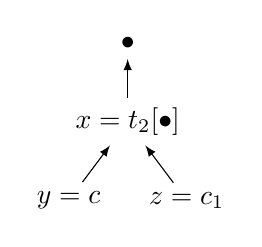
\begin{tikzpicture}[ 
  edge from parent path={(\tikzchildnode\tikzchildanchor) edge [-latex] (\tikzparentnode\tikzparentanchor)},
  level distance=1cm
]
\node (d) {$\bullet$} child{node (a) {$x=t_2[\bullet]$} child{node (b) {$y=c$}} child{node (c)
{$z=c_1$}}};

\end{tikzpicture}
\end{center}
Now each of the environments is represented by a linked list, with the binding
of $x$ shared between them. This is an example of a \emph{shared} environment
~\cite{appel1988optimizing}. This shared, linked structure dates back to the 
first machine for evaluating expressions, Landin's SECD
machine~\cite{landin1964mechanical}.

The drawbacks and advantages of each approach are well known. With a flat
environment, variable lookup can be performed with a simple offset
~\cite{jonesstg,appel1992compiling}. On the other hand, significant
duplication can occur, as we will discuss in Section~\ref{sec:exist}.
With a shared environment, that duplication is removed, but at the cost of
possible link traversal upon dereference. 

As with most topics in compilers and abstract machines, the design space is
actually more complex. For example, Appel and Jim show a wide range of hybrids
~\cite{appel1988optimizing} between the two, and Appel and Shao
~\cite{shao1994space} show an optimized hybrid that aims to achieve the benefits
of both approaches. And as shown in the next section, choice of evaluation
strategy further complicates the picture.

\section{Existing Call-by-Need Environments} \label{sec:exist}

Existing call by need machines use flat environments with a heap of
closures~\cite{jonesstg,TIM,johnsson1984efficient,boquist1997grin}. These
environments may contain some combination of primitive values and pointers into the
heap ($p$ below). The pointers and heap implement the memoization of results
required for call by need. Returning to the earlier example, $(\lambda
x.(\lambda y.t) (\lambda z.t_1)) t_2$, we can view a simplified execution state
for this approach when entering $t$ as follows:

\begin{center}
\textbf{Closure}
\begin{align*}
t[x=p_0, y=p_1] \\
\end{align*}
\textbf{Heap}
\begin{align*}
p_0 &\mapsto t_2[\bullet] \\
p_1 &\mapsto \lambda z.t_1[x=p_0] 
\end{align*}
\end{center}

Consider $t_2[\bullet]$, the closure at $p_0$. If it is not in WHNF (this sort
of unevaluated closure is called a
\emph{thunk}~\cite{ingerman1961way,peyton1992implementing}), then if it is
entered in either the evaluation of $t$ or $t_1$, the resulting value will
overwrite the closure at $p_0$. The result of the computation is then shared
with all other instances of $x$ in $t$ and $t_1$. In the case that terms have a
large number of shared variables, environment duplication can be expensive.
Compile-time transformation ~\cite{peyton1992implementing} (tupling arguments)
helps, but we show that the machine can avoid duplication completely.

Depending on $t$, either or both of the closures created for its free variables
may not be evaluated. Therefore, it is possible that the work of creating the
environment for that thunk will be wasted. This waste is well known, and
existing approaches address it by avoiding thunks as much as possible
~\cite{jonesstg,johnsson1984efficient}. Unfortunately, in cases like the above
example, thunks are necessary. We aim to minimize the cost of creating such
thunks.

Thunks are special in another way.  Recall that one advantage of flat
environments is quick variable lookups. In a lazy language, this advantage is
reduced because \emph{a thunk can only be entered once}. After it is entered, it
is overwritten with a value, so the next time that heap location is entered it
is entered with a value and a different environment. Thus, the work to ensure
that the variable lookup is fast is used only once. This is in contrast to
a call by value language, in which every closure is constructed for a value,
and can be entered an arbitrary number of times. 

A more subtle drawback of the flat environment representation is that
environments can vary in size, and thus a value in WHNF can be too large to fit
in the space allocated for the thunk it is replacing. This problem is discussed
in~\cite{jonesstg}, where the proposed solution is to put the value closure in
a fresh location in the heap where there is sufficient room. The original
thunk location is then replaced with an indirection to the value at the freshly
allocated location. These indirections are removed during garbage collection,
but do impose some cost, both in runtime efficiency and implementation
complexity~\cite{jonesstg}.

We have thus far ignored a number of details with regard to current
implementations. For example, the STG machine can split the flat environment, so
that part is allocated on the stack and part on the heap.  The TIM allocates its
flat environments separately from its closures so that each closure is a code
pointer, environment pointer pair~\cite{TIM} while the STG machine keeps
environment and code co-located~\cite{jonesstg}. Still, the basic design
principle holds: a flat environment for each closure allows quick variable
indexing, but with an initial overhead.

To summarize, the flat environment representation in a call by need language
implies that whenever a term might be needed, the necessary environment is
constructed from the current environment.  This operation can be expensive, and
it is wasted if the variable is never entered. In this work, we aim to minimize
this potentially unnecessary overhead.

Figure~\ref{fig:designspace} depicts the design space relevant to this chapter.
There are existing call by value machines with both flat and shared
environments, and call by need machines with flat environments. As far as we are
aware, we are the first to use a shared environment to implement lazy
evaluation. 

It is worth noting that there has been work on lazy machines that effectively use
linked environments, which could potentially be implemented as a shared
environment, e.g., Sestoft's work on Krivine machines~\cite{sestoft}, but none
make the realization that the shared environment can be used to implement
sharing of results, which is the primary contribution of this chapter.

\begin{figure}
\begin{tabularx}{\textwidth}{l | X | X}
                & Flat Environment     & Shared Environment \\ \hline
  Call by need  & STG~\cite{jonesstg}, 
                  TIM~\cite{TIM}, 
                  GRIN~\cite{boquist1997grin} 
                & $\mathcal{\mathcal{C} \mskip -4mu \mathcal{E}}$ Machine \\
  Call by value & ZAM~\cite{leroy1990zinc}, 
                  SML/NJ~\cite{appel1991standard}
                & ZAM,
                  SECD~\cite{landin1964mechanical}, 
                  SML/NJ \\
\end{tabularx}
\caption{Evaluation strategy and environment structure design space. Each
acronym refers to an existing implementation. Some implementations use multiple
environment representations.}
\label{fig:designspace}
\end{figure}

